\documentclass[aps,prl,reprint]{revtex4-2}

\usepackage{amsmath}
\usepackage{amssymb}
\usepackage{graphicx}
\usepackage{bm}
\usepackage{hyperref}
\usepackage{fancyhdr}

\pagestyle{fancy}
\fancyhf{}
\fancyhead[C]{\small Preprint -- Work in Progress}
\fancyfoot[R]{\small QuantumToy measurement-thickness preprint v0.2}
\renewcommand{\headrulewidth}{0pt}

\begin{document}

\title{Emergent Branch Selection and Finite Measurement Thickness in a Quantum Simulation Framework}

\author{Saku H\"am\"al\"ainen}

\date{\today}

\begin{abstract}
We investigate measurement-like behavior in a numerical quantum simulation
framework equipped with an emergent detector model but no explicit collapse term.
In baseline Schr\"odinger evolution, the wave field spreads through multiple
available paths and generates the expected interference structure at the screen.
However, the detector outputs are not observed as a passive sampling of the
continuous Born density. Instead, detection events cluster into a small number
of discrete branches.

This behavior suggests that branch selection can arise from detector dynamics,
coarse graining, and propagation geometry, even without introducing an explicit
nonlinear collapse operator into the wave evolution itself. The results further
indicate that the selection process is not pointlike in time. Rather, it appears
to develop over a finite spatiotemporal region, which we describe as a finite
measurement thickness.

We propose a geometric test configuration consisting of a wide slit followed by
a downstream double slit with variable separation distance. In this setup, the
distance between structures controls a transition between near-field, intermediate,
and far-field regimes. This provides a direct numerical probe of whether branch
selection is gradual and geometry dependent.

The framework does not claim to replace standard quantum mechanics. Instead, it
offers an exploratory computational model for studying how discrete detector
outcomes may emerge from continuous wave dynamics through a finite, structured,
measurement process.
\end{abstract}

\maketitle

\section{Introduction}

Quantum mechanics describes the evolution of a system through the Schr\"odinger
equation
\begin{equation}
i\hbar \partial_t \psi = H \psi.
\end{equation}
This unitary dynamics successfully predicts interference, diffraction, and a wide
range of experimentally verified phenomena. However, the relation between the
continuous wave description and the appearance of definite detection outcomes
remains conceptually nontrivial.

In standard textbook treatments, a measurement outcome is associated with the
Born rule, according to which the probability density is
\begin{equation}
\rho(\mathbf r,t)=|\psi(\mathbf r,t)|^2.
\end{equation}
This rule predicts outcome frequencies, but it does not by itself specify a
mechanism by which a single event becomes definite in an individual run.

The purpose of the present work is not to propose a new fundamental law of
quantum dynamics, but to explore a computational model in which discrete
measurement outcomes emerge from ordinary wave propagation together with a
structured detector model. The central question is not only \emph{which}
distribution is obtained, but \emph{how} branch selection develops.

Our numerical observations suggest two main points. First, detection outputs are
not always a direct passive sampling of the continuous Born density. Instead,
they often organize into a small number of discrete branches. Second, this
selection appears to occur gradually over a finite spatiotemporal region rather
than instantaneously at a single point. We refer to this as \emph{finite
measurement thickness}.

These observations motivate a new class of numerical experiments aimed at
probing where, when, and how branch selection occurs.

\section{Baseline wave evolution}

We begin from ordinary Schr\"odinger evolution in a two-dimensional geometry.
An initial Gaussian packet is propagated toward a barrier structure using a
split-operator method. In the absence of any detector-specific modification,
the evolution produces the familiar diffraction and interference patterns.

Forward evolution from an initial state $\psi_0$ is written as
\begin{equation}
\psi(\mathbf r,t)=U(t,t_0)\psi_0(\mathbf r).
\end{equation}
The corresponding Born density is
\begin{equation}
\rho(\mathbf r,t)=|\psi(\mathbf r,t)|^2.
\end{equation}

For a double-slit geometry, $\rho$ typically develops an interference pattern
downstream of the barrier. This continuous field structure serves as the
reference against which detector outputs are compared.

\section{Emergent detector model}

The detector model considered here is intentionally exploratory. It does not
insert an explicit collapse term into the Schr\"odinger equation. Instead,
discrete outcomes are extracted from the evolving field by a structured
detection process involving finite spatial resolution, local maxima selection,
and branch-like clustering of clicks.

At the most general level, the detector is represented by a map
\begin{equation}
\mathcal D : \psi(\mathbf r,t) \mapsto \{ y_i \},
\end{equation}
where $\{y_i\}$ is a set of discrete detection positions at the screen.
This map may depend on local density structure, neighborhood information,
thresholding, and detector geometry.

The key point is that the detector is not modeled as an infinitesimal passive
sampler of $\rho$. It is instead a coarse-grained, finite-resolution operation
acting on the propagated field.

\section{Observed branch selection}

A central numerical observation is that the detector output may differ
qualitatively from the raw Born density. In several runs, the Born density
along the detector line exhibits multiple peaks and fine structure, while the
actual click events cluster into a much smaller number of narrow horizontal
bands.

This suggests the following distinction:
\begin{itemize}
\item the wave field remains spatially extended and may pass through multiple
available paths,
\item but the detector outputs organize into a discrete set of branches.
\end{itemize}

A useful empirical representation of the click distribution is
\begin{equation}
P_{\mathrm{click}}(y) \approx \sum_{k} w_k \, \delta(y-y_k),
\end{equation}
where $y_k$ are branch centers and $w_k$ are empirical branch weights.

The appearance of such discrete branch bands, even when the underlying Born
density is continuous and structured, indicates that branch selection can arise
from the detector process itself. In this sense, the detector acts as a
nontrivial coarse-graining operation rather than a transparent readout of
$|\psi|^2$.

\section{Born peaks versus emergent branch centers}

A more detailed comparison reveals that the branch centers need not coincide
with the maxima of the Born density. Figure~\ref{fig:bornpeakcomparison}
shows a representative case from a $400$-click simulation. The continuous
Born screen density is shown together with the empirical click histogram and
the automatically extracted branch centers.

\begin{figure}[t]
\centering
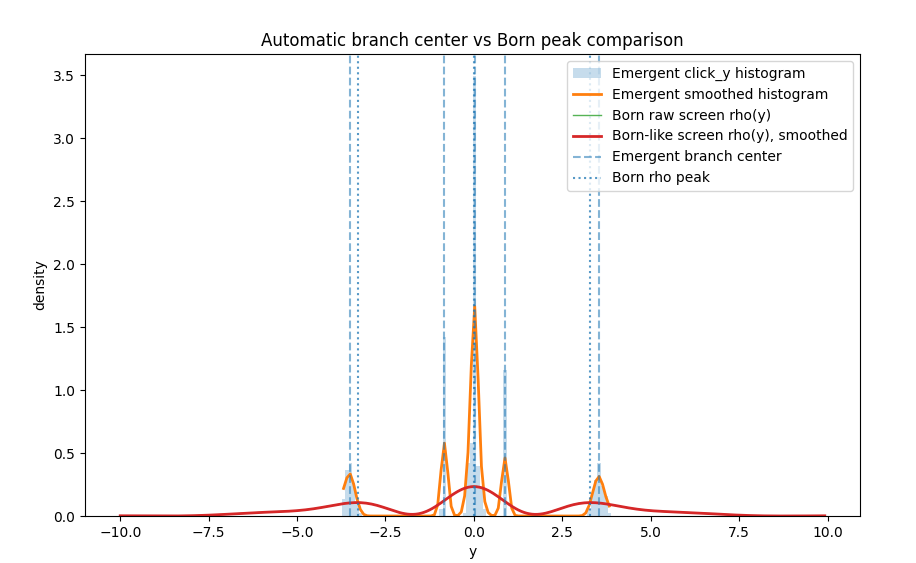
\includegraphics[width=\linewidth]{born_peak_comparison.png}
\caption{
Comparison between the continuous Born density and the discrete detector output.
The red curve shows the smoothed Born density at the screen.
The blue histogram and orange curve represent the empirical distribution of detection events.
}
\label{fig:bornpeakcomparison}
\end{figure}

The comparison in Fig.~\ref{fig:bornpeakcomparison} is important for two
reasons. First, it shows that the detector output is much sharper than the
underlying Born profile. Second, it shows that one broad Born lobe can
correspond to several distinct outcome branches. The detector therefore appears
to generate its own effective attractor structure rather than merely reading
out preexisting Born maxima.

This observation supports the view that measurement-like selection in the
present framework is a structural dynamical process. The result is not simply a
continuous density sampled at random, but a small set of stable, discrete
outcome channels arising from coarse graining, propagation, and detector
geometry.

\section{Field-level superposition versus branch-level outcome}

The numerical results support a distinction between two levels of description.

First, at the field level, the wave function remains extended and may occupy
multiple geometrically available paths simultaneously. In this sense, the
simulation exhibits the ordinary superpositional character of wave dynamics.

Second, at the branch level, the detector output does not retain the full
continuous support of the field. Instead, it selects a discrete subset of
stable outcome channels.

This suggests the following qualitative interpretation:
\begin{equation*}
\psi \;\longrightarrow\; \rho=|\psi|^2
\end{equation*}
\begin{equation}
\;\longrightarrow\; \text{detector coarse graining}
\;\longrightarrow\; \text{discrete branches}.
\end{equation}

The distinction is important. The field may remain extended across multiple
paths, while the observed click is localized to a single branch. The present
framework therefore does not treat the localized outcome as identical to the
full wave field itself.

\section{Finite measurement thickness}

The most important conceptual proposal of this work is that branch selection
may possess a finite spatiotemporal thickness. In other words, the transition
from extended superposition to effective branch selection may occur over an
interval rather than at a mathematical instant.

We express this schematically by introducing a selection interval
\begin{equation}
t \in [t_1,t_2],
\end{equation}
during which the propagated field, the geometry, and the detector collectively
drive the system toward an effectively discrete outcome structure.

In this picture, measurement is not modeled as a singular event at a single
time slice. Instead, it is a gradual process whose effective thickness depends
on propagation distance, diffraction regime, and detector structure.

\section{Wide-slit to double-slit transition geometry}

To probe this idea, we propose a numerical experiment consisting of a wide slit
followed by a downstream double slit:
\begin{equation}
\text{source} \rightarrow \text{wide slit} \rightarrow
\text{distance }L \rightarrow \text{double slit} \rightarrow \text{screen}.
\end{equation}

The distance $L$ between the wide slit and the downstream double slit is the
control parameter. This geometry is particularly useful because it naturally
interpolates between three regimes:

\subsection{Near-field regime}

For small $L$, the wave packet has little time to spread after the wide slit.
The downstream double slit then behaves approximately like a solid central
obstacle with limited effective path separation. In this regime, the field may
remain strongly centered and branch selection may already be partially advanced
before the second structure becomes effective.

\subsection{Far-field regime}

For large $L$, the field has time to diffract substantially before reaching the
double slit. The second barrier then acts on a broader incoming field, and the
usual double-slit interference structure is expected to re-emerge more fully.

\subsection{Intermediate regime}

The most interesting case is intermediate $L$, where the field is neither
strongly localized nor fully spread. In this transition region, branch
selection may be partial, unstable, or multi-stage. This is precisely the
regime in which a finite measurement thickness should become visible if the
selection process is truly gradual.

\section{Quantitative diagnostics}

Several numerical diagnostics are useful for characterizing branch selection in
this framework.

\subsection{Branch count}

If click events cluster around branch centers $y_k$, the effective number of
branches may be estimated from the number of robust histogram peaks or from
cluster extraction methods applied to the click coordinates.

\subsection{Interference visibility}

A standard measure of fringe visibility at the screen is
\begin{equation}
V=\frac{I_{\max}-I_{\min}}{I_{\max}+I_{\min}},
\end{equation}
where $I_{\max}$ and $I_{\min}$ are representative neighboring maxima and minima
of the screen intensity.

\subsection{Selection stability}

A branch trajectory extracted from local maxima or ridge tracking may be used to
quantify how early a branch becomes stable. If a branch coordinate $y_R(t)$
locks into a narrow channel before the detector region is reached, this supports
the interpretation that selection develops upstream of the final click event.

\subsection{Born-to-click deviation}

The difference between the raw Born density and the click histogram is itself an
important observable. If the detector output is not a direct sampling of the
screen density, then
\begin{equation}
P_{\mathrm{click}}(y) \neq C\,\rho_{\mathrm{screen}}(y)
\end{equation}
for any simple proportionality constant $C$.

\section{Phase structure and branch structure}

Additional diagnostics compare branch structure with phase structure.
In the present simulations, branch locations do not appear to follow raw phase
stripes directly. Instead, they seem to reflect a combination of amplitude
envelope, local geometry, propagation history, and detector coarse graining.

This observation is important because it argues against the oversimplified idea
that each branch is merely a direct image of a phase domain. Instead, the
detector appears to extract stable outcome bands from the combined wave
structure, rather than from phase alone.

\section{Relation to other viewpoints}

The present framework is exploratory and sits conceptually between several
familiar viewpoints.

Compared with standard textbook measurement, it attempts to model the emergence
of a definite outcome as a process rather than taking collapse as primitive.

Compared with Bohmian mechanics, it shares the distinction between an extended
wave field and localized effective outcomes, but it does not introduce a full
ontological particle trajectory law of Bohmian type.

Compared with decoherence-inspired viewpoints, it emphasizes that a structured
detector and propagation geometry may themselves generate effective branch
selection and coarse graining.

The present work does not claim equivalence to any of these interpretations.
Its aim is more modest: to provide a numerical framework in which finite
selection thickness can be studied explicitly.

\section{Limitations}

Several limitations should be emphasized.

\begin{itemize}
\item The detector model is phenomenological and not derived from a microscopic
detector Hamiltonian.

\item Numerical results depend on grid resolution, threshold choices, and branch
extraction methods.

\item The present framework has not yet been calibrated against laboratory
detector response functions.

\item The model does not by itself establish a new fundamental interpretation of
quantum theory; it only demonstrates that discrete branch-like outputs can
emerge in an explicit simulation framework without an inserted collapse term.
\end{itemize}

\section{Conclusion}

We have explored a numerical framework in which wave propagation remains
continuous, but detector outputs become organized into discrete branches.
These observations suggest that measurement-like behavior can emerge from the
combination of extended wave dynamics, detector coarse graining, and propagation
geometry, even without an explicit collapse operator.

The results motivate the idea of \emph{finite measurement thickness}: branch
selection may occur gradually over a finite spatiotemporal region rather than
at a single instant. A proposed wide-slit-to-double-slit geometry with variable
separation distance provides a direct way to probe this transition numerically.

The comparison between Born maxima and emergent branch centers shows that the
detector output is not simply a sharpened copy of the Born distribution. Instead,
the detector appears to generate discrete outcome channels with their own
effective branch structure.

The framework is exploratory, but it offers a concrete path for studying how
definite detector outcomes may emerge from continuous quantum evolution through
structured branch selection processes.

\begin{thebibliography}{9}

\bibitem{quantumtoy}
S.~H\"am\"al\"ainen,
\href{https://github.com/placeholder/quantumtoy}{QuantumToy code repository}
(placeholder URL).

\bibitem{trf}
S.~H\"am\"al\"ainen,
``Thick Reality Front: a numerical framework for spacetime structure in quantum evolution,''
unpublished preprint.

\bibitem{bohm}
D.~Bohm,
``A Suggested Interpretation of the Quantum Theory in Terms of `Hidden' Variables. I,''
Phys.\ Rev.\ \textbf{85}, 166 (1952).

\bibitem{zurek}
W.~H.~Zurek,
``Decoherence, einselection, and the quantum origins of the classical,''
Rev.\ Mod.\ Phys.\ \textbf{75}, 715 (2003).

\end{thebibliography}

\end{document}